% Options for packages loaded elsewhere
\PassOptionsToPackage{unicode}{hyperref}
\PassOptionsToPackage{hyphens}{url}
\PassOptionsToPackage{dvipsnames,svgnames,x11names}{xcolor}
%
\documentclass[
  letterpaper,
  DIV=11,
  numbers=noendperiod]{scrartcl}

\usepackage{amsmath,amssymb}
\usepackage{iftex}
\ifPDFTeX
  \usepackage[T1]{fontenc}
  \usepackage[utf8]{inputenc}
  \usepackage{textcomp} % provide euro and other symbols
\else % if luatex or xetex
  \usepackage{unicode-math}
  \defaultfontfeatures{Scale=MatchLowercase}
  \defaultfontfeatures[\rmfamily]{Ligatures=TeX,Scale=1}
\fi
\usepackage{lmodern}
\ifPDFTeX\else  
    % xetex/luatex font selection
\fi
% Use upquote if available, for straight quotes in verbatim environments
\IfFileExists{upquote.sty}{\usepackage{upquote}}{}
\IfFileExists{microtype.sty}{% use microtype if available
  \usepackage[]{microtype}
  \UseMicrotypeSet[protrusion]{basicmath} % disable protrusion for tt fonts
}{}
\makeatletter
\@ifundefined{KOMAClassName}{% if non-KOMA class
  \IfFileExists{parskip.sty}{%
    \usepackage{parskip}
  }{% else
    \setlength{\parindent}{0pt}
    \setlength{\parskip}{6pt plus 2pt minus 1pt}}
}{% if KOMA class
  \KOMAoptions{parskip=half}}
\makeatother
\usepackage{xcolor}
\setlength{\emergencystretch}{3em} % prevent overfull lines
\setcounter{secnumdepth}{-\maxdimen} % remove section numbering
% Make \paragraph and \subparagraph free-standing
\ifx\paragraph\undefined\else
  \let\oldparagraph\paragraph
  \renewcommand{\paragraph}[1]{\oldparagraph{#1}\mbox{}}
\fi
\ifx\subparagraph\undefined\else
  \let\oldsubparagraph\subparagraph
  \renewcommand{\subparagraph}[1]{\oldsubparagraph{#1}\mbox{}}
\fi


\providecommand{\tightlist}{%
  \setlength{\itemsep}{0pt}\setlength{\parskip}{0pt}}\usepackage{longtable,booktabs,array}
\usepackage{calc} % for calculating minipage widths
% Correct order of tables after \paragraph or \subparagraph
\usepackage{etoolbox}
\makeatletter
\patchcmd\longtable{\par}{\if@noskipsec\mbox{}\fi\par}{}{}
\makeatother
% Allow footnotes in longtable head/foot
\IfFileExists{footnotehyper.sty}{\usepackage{footnotehyper}}{\usepackage{footnote}}
\makesavenoteenv{longtable}
\usepackage{graphicx}
\makeatletter
\def\maxwidth{\ifdim\Gin@nat@width>\linewidth\linewidth\else\Gin@nat@width\fi}
\def\maxheight{\ifdim\Gin@nat@height>\textheight\textheight\else\Gin@nat@height\fi}
\makeatother
% Scale images if necessary, so that they will not overflow the page
% margins by default, and it is still possible to overwrite the defaults
% using explicit options in \includegraphics[width, height, ...]{}
\setkeys{Gin}{width=\maxwidth,height=\maxheight,keepaspectratio}
% Set default figure placement to htbp
\makeatletter
\def\fps@figure{htbp}
\makeatother

\KOMAoption{captions}{tableheading}
\makeatletter
\@ifpackageloaded{caption}{}{\usepackage{caption}}
\AtBeginDocument{%
\ifdefined\contentsname
  \renewcommand*\contentsname{Table of contents}
\else
  \newcommand\contentsname{Table of contents}
\fi
\ifdefined\listfigurename
  \renewcommand*\listfigurename{List of Figures}
\else
  \newcommand\listfigurename{List of Figures}
\fi
\ifdefined\listtablename
  \renewcommand*\listtablename{List of Tables}
\else
  \newcommand\listtablename{List of Tables}
\fi
\ifdefined\figurename
  \renewcommand*\figurename{Figure}
\else
  \newcommand\figurename{Figure}
\fi
\ifdefined\tablename
  \renewcommand*\tablename{Table}
\else
  \newcommand\tablename{Table}
\fi
}
\@ifpackageloaded{float}{}{\usepackage{float}}
\floatstyle{ruled}
\@ifundefined{c@chapter}{\newfloat{codelisting}{h}{lop}}{\newfloat{codelisting}{h}{lop}[chapter]}
\floatname{codelisting}{Listing}
\newcommand*\listoflistings{\listof{codelisting}{List of Listings}}
\makeatother
\makeatletter
\makeatother
\makeatletter
\@ifpackageloaded{caption}{}{\usepackage{caption}}
\@ifpackageloaded{subcaption}{}{\usepackage{subcaption}}
\makeatother
\ifLuaTeX
  \usepackage{selnolig}  % disable illegal ligatures
\fi
\usepackage{bookmark}

\IfFileExists{xurl.sty}{\usepackage{xurl}}{} % add URL line breaks if available
\urlstyle{same} % disable monospaced font for URLs
\hypersetup{
  pdftitle={Analyse et Traitement Avancé des Données avec R},
  pdfauthor={PEHAN Boré Hermann},
  colorlinks=true,
  linkcolor={blue},
  filecolor={Maroon},
  citecolor={Blue},
  urlcolor={Blue},
  pdfcreator={LaTeX via pandoc}}

\title{Analyse et Traitement Avancé des Données avec R}
\author{PEHAN Boré Hermann}
\date{}

\begin{document}
\maketitle

\subsection{Introduction à R et
Rstudio}\label{introduction-uxe0-r-et-rstudio}

\subsubsection{R}\label{r}

\begin{itemize}
\item
  Logiciel open-source
\item
  Langage orienté vers le traitement, l'analyse des données et que la
  visualisation des données
\item
  Rédaction de rapport (word, powerpoint, pdf et html)
\item
  Installation

  \begin{itemize}
  \tightlist
  \item
    Sous windows:
    \href{http://cran.r-project.org/bin/windows/base/}{Télécharger ici}
  \item
    Sous Mac OS X:
    \href{http://cran.r-project.org/bin/macosx/}{Télécharger ici}
  \end{itemize}
\end{itemize}

\subsubsection{Rstudio}\label{rstudio}

\begin{itemize}
\item
  Environnement de développement intégré pour R
\item
  Installation:
  \href{http://www.rstudio.com/products/rstudio/download/}{Télécharger
  ici}
\end{itemize}

\subsection{Importation de fichier}\label{importation-de-fichier}

\subsubsection{Importation des fichiers textes
(.txt,.csv)}\label{importation-des-fichiers-textes-.txt.csv}

\paragraph{Importation graphique}\label{importation-graphique}

\begin{figure}[H]

{\centering 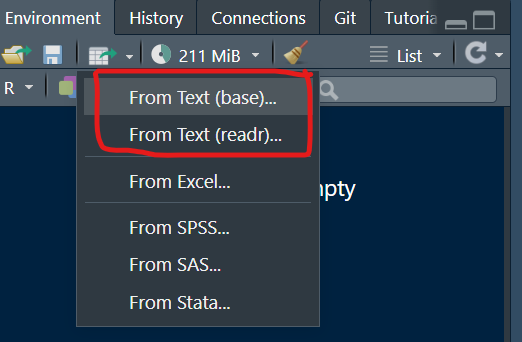
\includegraphics{images/importation_interface.png}

}

\caption{Charger un fichier texte par l'interface}

\end{figure}%

\subsection{Introduction à la gestion avancée des données avec
R}\label{introduction-uxe0-la-gestion-avancuxe9e-des-donnuxe9es-avec-r}

\subsubsection{Lecture des données}\label{lecture-des-donnuxe9es}

\subsubsection{\texorpdfstring{Concepts avancés de manipulation des
données avec \texttt{tidyverse} et
\texttt{data.table}}{Concepts avancés de manipulation des données avec tidyverse et data.table}}\label{concepts-avancuxe9s-de-manipulation-des-donnuxe9es-avec-tidyverse-et-data.table}

\paragraph{\texorpdfstring{Concepts avancés de manipulation des données
avec
\texttt{tidyverse}}{Concepts avancés de manipulation des données avec tidyverse}}\label{concepts-avancuxe9s-de-manipulation-des-donnuxe9es-avec-tidyverse}

\paragraph{\texorpdfstring{Concepts avancés de manipulation des données
avec
\texttt{data.table}}{Concepts avancés de manipulation des données avec data.table}}\label{concepts-avancuxe9s-de-manipulation-des-donnuxe9es-avec-data.table}

\subsubsection{Optimisation du traitement des grands ensembles de
données}\label{optimisation-du-traitement-des-grands-ensembles-de-donnuxe9es}

\subsubsection{Programmation fonctionnelle et manipulation efficace des
données}\label{programmation-fonctionnelle-et-manipulation-efficace-des-donnuxe9es}

\subsection{Analyse exploratoire et
modélisation}\label{analyse-exploratoire-et-moduxe9lisation}

\subsubsection{\texorpdfstring{Techniques avancées de visualisation avec
\texttt{ggplot2} et
\texttt{plotly}}{Techniques avancées de visualisation avec ggplot2 et plotly}}\label{techniques-avancuxe9es-de-visualisation-avec-ggplot2-et-plotly}

\subsubsection{\texorpdfstring{Méthodes statistiques et modélisation
prédictive avec \texttt{caret} et
\texttt{randomForest}}{Méthodes statistiques et modélisation prédictive avec caret et randomForest}}\label{muxe9thodes-statistiques-et-moduxe9lisation-pruxe9dictive-avec-caret-et-randomforest}

\subsubsection{\texorpdfstring{Analyse des séries temporelles avec
\texttt{forecast}}{Analyse des séries temporelles avec forecast}}\label{analyse-des-suxe9ries-temporelles-avec-forecast}

\subsection{Traitement des données et
automatisation}\label{traitement-des-donnuxe9es-et-automatisation}

\subsubsection{\texorpdfstring{Automatisation du nettoyage des données
avec
\texttt{tidymodels}}{Automatisation du nettoyage des données avec tidymodels}}\label{automatisation-du-nettoyage-des-donnuxe9es-avec-tidymodels}

\subsubsection{\texorpdfstring{Optimisation des performances d'analyse
avec \texttt{parallel} et
\texttt{bigmemory}}{Optimisation des performances d'analyse avec parallel et bigmemory}}\label{optimisation-des-performances-danalyse-avec-parallel-et-bigmemory}

\subsubsection{\texorpdfstring{Interaction entre R et Python avec
\texttt{reticulate}}{Interaction entre R et Python avec reticulate}}\label{interaction-entre-r-et-python-avec-reticulate}



\end{document}
